\section{はじめに}
ゲーム産業は娯楽産業の中でも大きな収益を上げている産業であり、2019年の世界ゲームコンテンツ市場の規模は15兆6898億円と推定されている\cite{prtimes}。国内でもゲーム産業は10年連続で成長しており、市場規模は1兆7330億円となっている。その中でも家庭用ハードや家庭用ソフトと比較して、スマートフォンのアプリやPC向けのオンラインゲームのゲームの市場規模が年々拡大している。このようにゲームのプレイスタイルがゲーム専用機を購入するというものから汎用端末でのゲームプレイへと変化を見せている。こういった状況下で注目されている新たな手法で展開されるゲームサービスの一つにクラウドゲーミングがある。

従来のゲームプレイは、プレイヤーがゲーム専用機やゲーミングPC等を所有し、その上でゲームを動作させることによって実現されている。一方、クラウドゲーミングにおいては、図\ref{fig:cloudgaming}のようにクラウドサーバ上でゲームを動作させてその画面をプレイヤーの端末にストリーミングすることで、ゲームをネットワーク越しにプレイすることを可能にしている。このとき、プレイヤーがゲームプレイに使用する端末は、クラウドサーバより送信されるゲーム画面の再生とプレイヤーの操作のサーバへの送信のみを行う。この仕組みによって、スマートフォンやタブレット等の性能が貧弱な端末でも、従来は高価なゲーム専用機やゲーミングPCを使用しなければ体験できなかった高品質なゲーム体験を得られる。

\begin{figure*}[t]
    \centering
    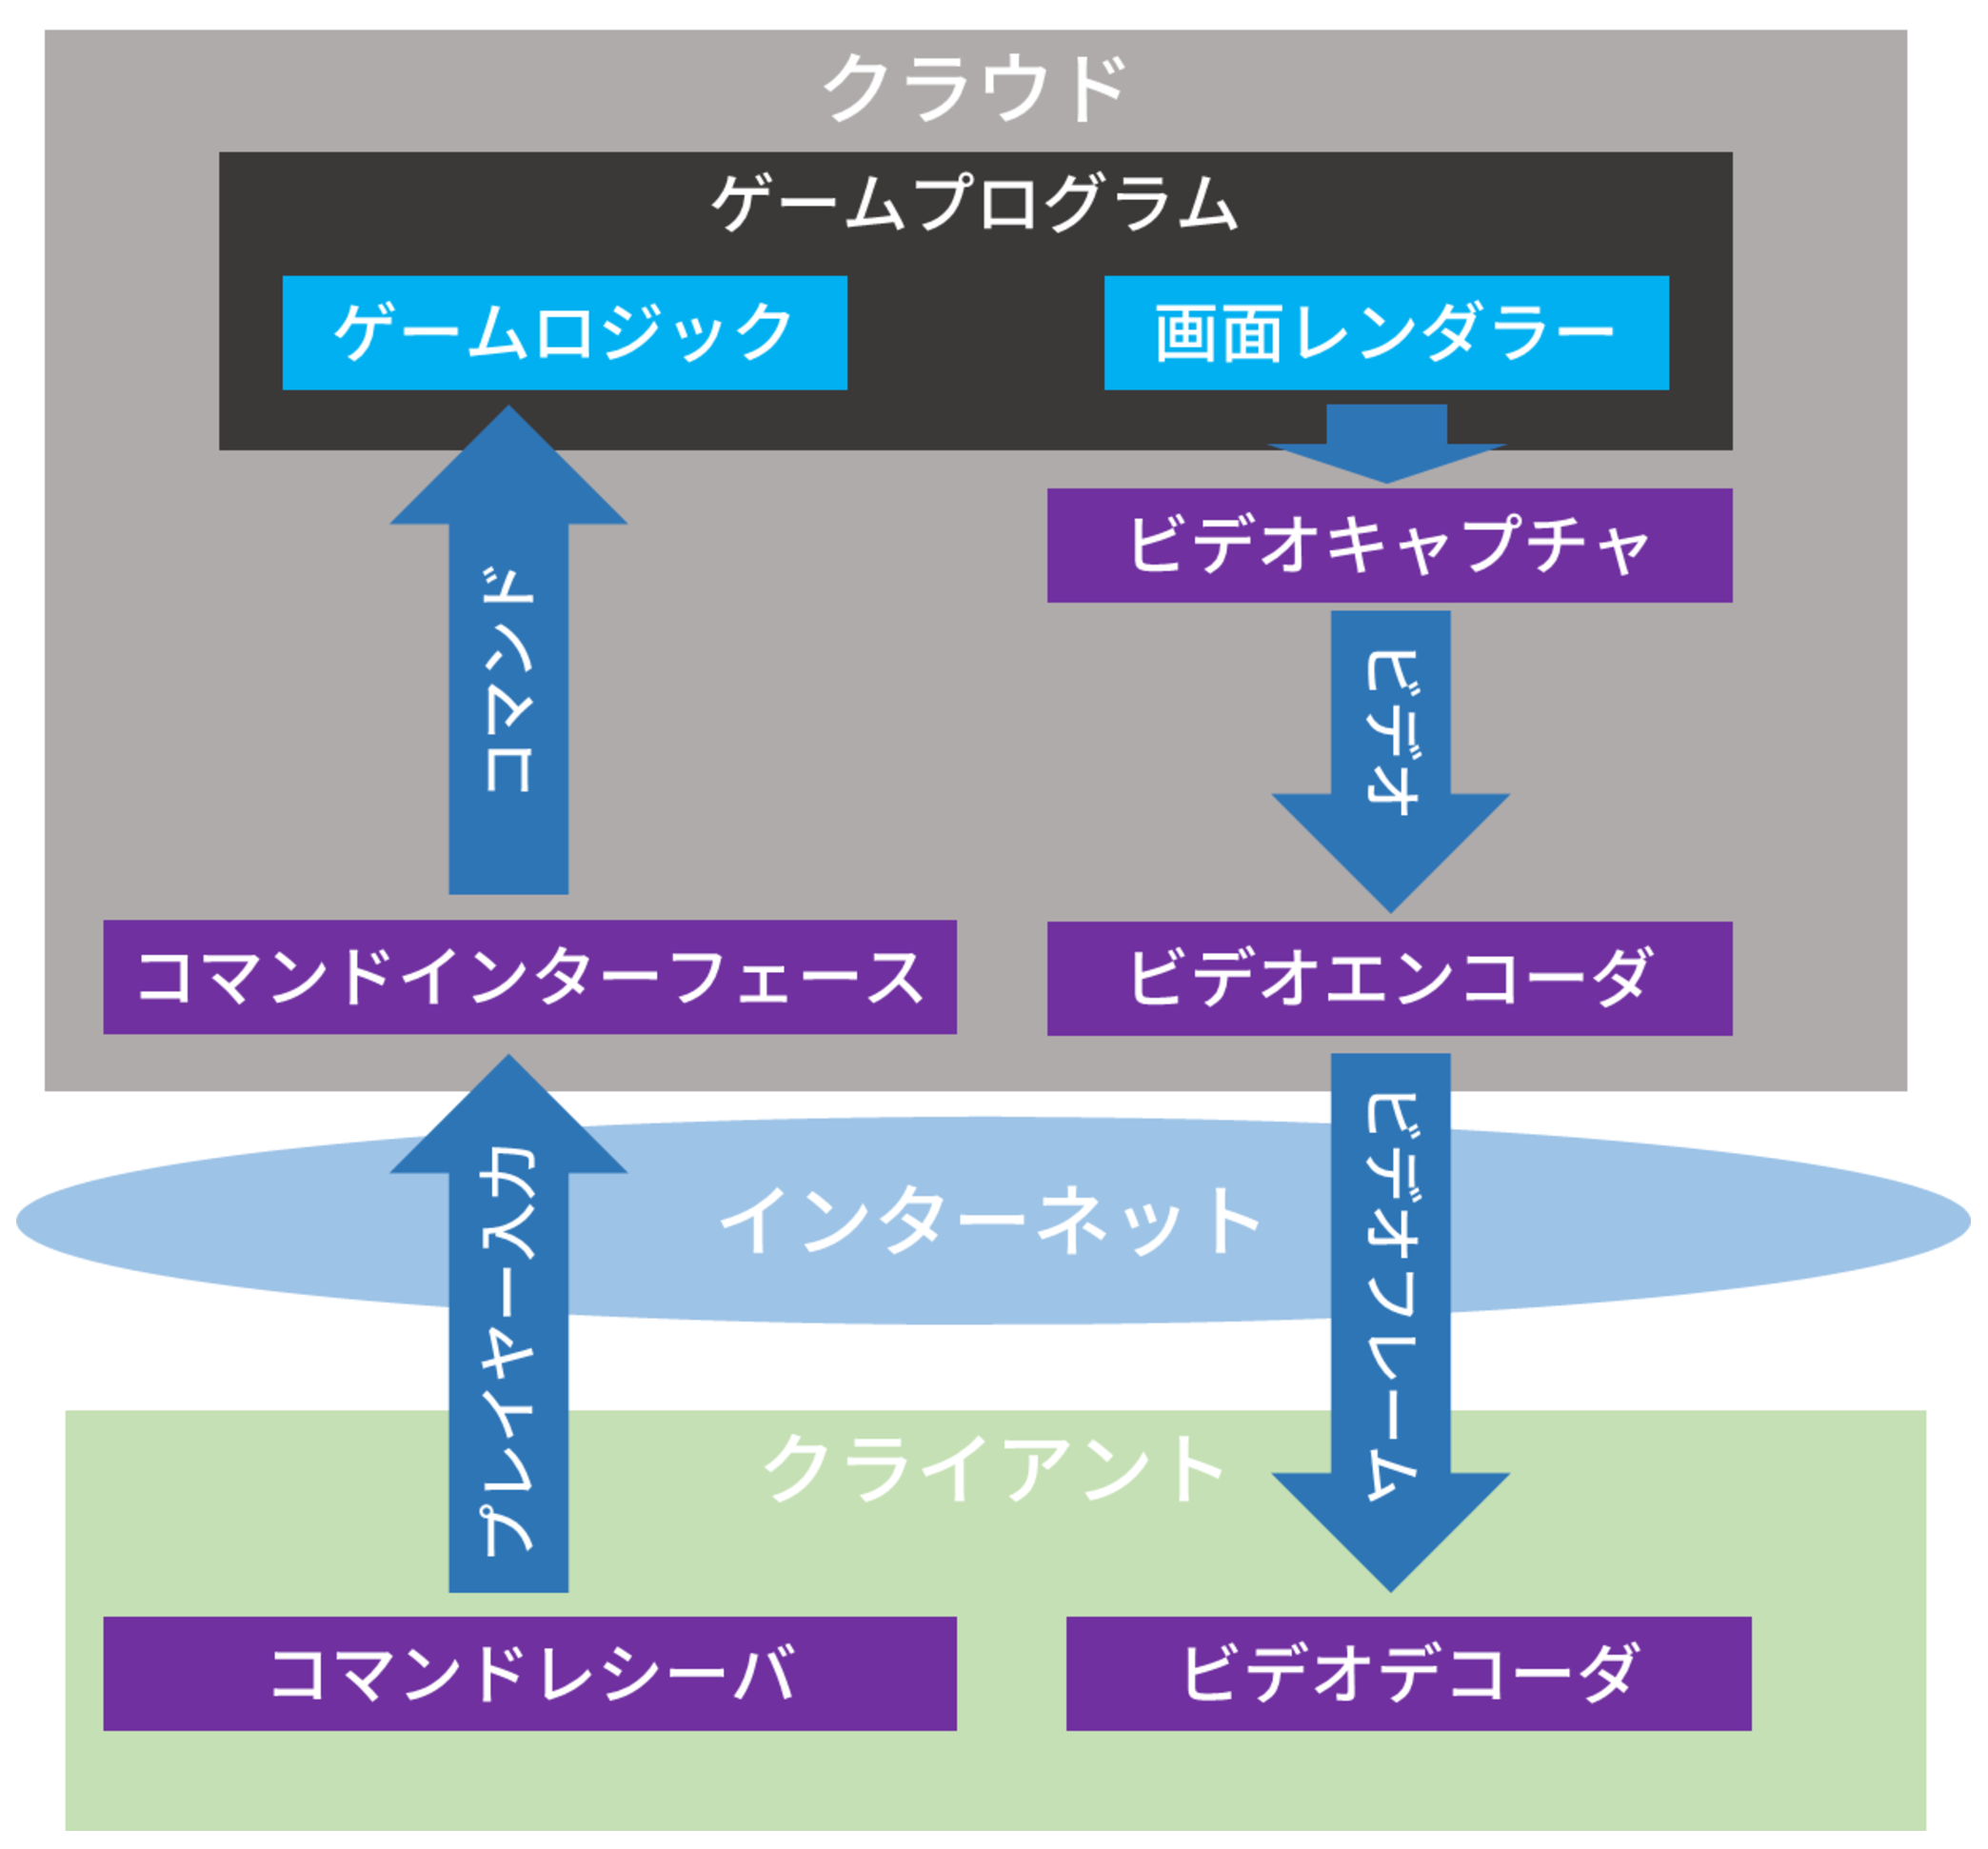
\includegraphics[width=0.8\textwidth,keepaspectratio,clip]{img/cloudgaming.eps}
    \caption{クラウドゲーミングプラットフォーム}
    \label{fig:cloudgaming}
\end{figure*}

クラウドゲーミングは既に商用サービスとして提供されている。過去には英国のOnLive\cite{onlive}やアメリカのGaikaiがクラウドゲーミングサービスを展開していた。これらは既にサービスを終了しているが、ソニーが2012年にGaikaiを買収し、2015年にサービスを閉鎖したOnLiveの資産を取得した\cite{onlive-sony-gaikai}。同年に、ソニーは新たにクラウドゲーミングサービスのPlayStation Now\cite{ps-now}を開始した。また、Googleも2019年にクラウドゲーミングサービスであるGoolge Stadia\cite{stadia}を開始した。Google Stadiaは同社のウェブブラウザであるGoogle Chromeをインターフェースとしているのが特徴で、ユーザーへのメディアのストリーミングに動画配信サービスのYouTubeを使用している。Google Stadiaは現在日本を含まない14カ国で展開されている。また、GPUのメーカーとして知られるNVIDIAが提供するクラウドゲーミングサービスGeForce NOW\cite{geforce-now}は、従来PCゲームをプレイしていたプレイヤー層をメインターゲットに据えており、PCゲーマーからの注目を集めている。他に、MicrosoftのProject xCloudやAmazonのLunaが海外でサービス開始されている。

商用サービスだけでなく、研究開発用のクラウドゲーミングプラットフォームも存在する。Huangら\cite{gaminganywhere}は、既存のクローズドソースのシステムでは研究開発のための修正や拡張を行うことが困難であることから、オープンソースのクラウドゲーミングプラットフォームであるGamingAnywhereを開発した。GamingAnywhereはWindows、Linux、macOS上で実装されており、クライアントはiOSやAndroid等の他のOSにも容易に移植が可能である。また、GamingAnywhereは詳細な設定を可能にしていて、更にオープンソースであるため拡張的な実装が可能であるなど、クラウドゲーミングに関する研究のテストベッドの構築に適している。

従来のゲームシステムとは一線を画するクラウドゲーミングには、依然として重要な課題が存在している\cite{cloudgaming-survey}。クラウドゲーミングサービスの提供者の視点から見た課題としては、ゲーム環境の仮想化やサーバにおける負荷分散といった課題がある。一方、クラウドゲーミングシステムのユーザであるプレイヤーの視点から見た課題としては、ゲーム体験の品質、すなわちQuality of Experience (QoE) がある。クラウドゲーミングにおけるQoEの担保に必要な課題としては、以下がある。
\begin{itemize}
    \item ストリーミングされるゲーム画面のレンダリング品質の担保
    \item ゲーム画面のリアルタイムストリーミングに耐えうる、充分なネットワーク帯域の確保
    \item 高圧縮率と高画質を両立する動画ストリーミングコーデックの実現
    \item プレイヤーによる操作が画面に反映されるまでの遅延の最小化
\end{itemize}

これらの課題の中でもプレイヤーの操作に対する応答性に直結する遅延の最小化は特に重要な課題である。Raaen\cite{delay}らの調査によると、一部のゲーマーは40ms未満のゲームの応答遅延を認識可能であり、また半数のゲーマーが100ms以上のの応答遅延を許容できないということが観測されている。
%動画配信プラットフォームにおけるライブストリーミングの場合、途切れることなく安定した動画の配信を行うためにバッファリングを行うことで対処する場合がある。しかしクラウドゲーミングは多くの場合、リアルタイムかつインタラクティブな性質を持つコンテンツであるためこの方法を使用することができない。
クラウドゲーミングサービスにおける応答時間は主に以下で構成される。
\begin{itemize}
    \item クライアント/サーバ間のネットワーク遅延
    \item サーバにおけるゲーム画面のレンダリング処理時間
    \item 動画ストリームのエンコード・デコード処理時間
\end{itemize}
これらの中でもネットワーク遅延が支配的であり、Lee\cite{outatime}らはネットワークのRTTが128msである場合、応答時間の約8割をネットワーク遅延が占めると指摘している。
そのため、クラウドサーバ上でのゲーム画面生成の高速化/効率化や、伝送データの圧縮、ネットワーク遅延の最小化などが課題となっている。

クラウドサービスを提供するサーバが配備されるデータセンターは、通常国内には数箇所しか存在しない。既存のクラウドゲーミングアーキテクチャにおいては、クラウドのサーバ上でゲームが動作している。このため、データセンターから地理的に遠いプレイヤーの端末からクラウドゲーミングサービスに接続するとネットワーク遅延が大きくなってしまうという問題がある。これがゲームプレイにおける応答遅延を増大させることとなり、プレイヤーのQoE低下の原因となり得る。データセンターに計算機資源を集約する現在のクラウドアーキテクチャを利用する限り、この遅延を解消することはできない。プレイヤーとクラウド上の計算機資源との間の物理的距離に起因する遅延を解消するためには、プレイヤーの地理的近傍に計算機資源を設置することが必要である。そのため、中央集権的なクラウドデータセンターのようなアーキテクチャの利用ではなく、広域に分散した計算機資源を活用する必要があると考えられる。

広域分散した計算機資源の活用形態としては、エッジコンピューティングや一般ユーザがボランティアとして計算機資源を提供するボランティアコンピューティングなどの活用が考えられる。しかしながら、エッジコンピューティングは一般的にIoTアプリケーションなどで用いられる比較的小規模な計算機資源であることから、クラウドゲーミングの用途には適さないと考えられる。一方で、一般ユーザが計算機を提供するボランティアコンピューティングは、大規模な科学技術計算を多数の小規模なタスクに分割して分散処理するべくして設計されたもので、ゲームをホストするために十分な計算機性能を確保できると考えられる。現在までに、SETI@home\cite{setiathome}やFolding@home\cite{folding}に代表されるボランティアコンピューティングプロジェクトが、高エネルギー物理学、分子生物学、医学、天体物理学、気候研究などの分野の研究で利用された。既存のクラウドコンピューティングの枠組みにおいては、クラウドサーバに一極集中した計算機資源にユーザがアクセスして利用する。それに対し、ボランティアコンピューティングにおいては、広域に分散した一般ユーザーのリソースを活用するという特徴がある。国内に数箇所しか存在しないクラウドのデータセンターに比べて、広域に分散した一般ユーザーの計算機資源は地理的に近傍である可能性が高い。この性質を利用し、よりネットワーク遅延の小さい計算機同士での通信でクラウドゲーミングを行えば、遅延の問題を解消する可能性がある。

本研究では、ボランティアが提供する地理的に近傍の遊休コンピュータを活用することによるクラウドゲーミングシステムを提案する。
%既存のクラウドゲーミングアーキテクチャにおいては、クラウドのサーバ上でゲームが動作しているため、プレイヤーの端末からデータセンターまでのネットワーク遅延を回避することは不可能である。国内のデータセンターまでのネットワーク遅延は最大50ms程度と言われている。これはゲームプレイにおけるレスポンスの遅延としては無視できない値であり、著しくプレイヤーのQoE低下の原因となり得る。
本研究では、プレイヤーの端末からデータセンターまでのネットワーク遅延を削減し、プレイヤーがクラウドゲーミングのプレイを通して体験する画面表示や操作の反映の遅延を最小化することでのプレイヤーのQoEの向上を目的とする。広域に分散したボランティアの提供する遊休コンピュータの中から、プレイヤーの端末から見て地理的に近傍のものを選択し、その上でクラウドゲームサーバを動作させる。これによって遅延の削減を目指す。

本論文の以後の部分は次のように構成されている。2章では、研究の背景と関連研究について述べる。3章では、提案システムの設計について述べる。4章では、提案システムの実装について述べる。5章では、提案システムの性能評価について述べる。6章では、まとめと今後の展望について述べる。







 
